\section{Carbon Fiber Filament}

\indent

In order to print the CFRP material, carbon fiber and a resin were combined into a CFRP filament. As in conventional FDM printing, the CFRP filament is extruded by driving it through a heated nozzle. ABS plastic was chosen as the matrix material for this filament for several reasons. First, ABS has already successfully been combined with chopped carbon fiber in FDM filaments. Second, ABS does not require post-processing to reach full strength, as epoxy-based pre-impregnated carbon fiber composites do. In all filament development methods a 1K carbon fiber tow (shown in Figure~\ref{fig:carbon-fiber-spool}) was utilized.\\

\begin{figure}[htp]
    \centering
    \includegraphics[width=0.5\textwidth]{./figures/carbon-fiber-spool}
    \caption{The 1K carbon fiber spool.}
    \label{fig:carbon-fiber-spool}
\end{figure}

\subsection{Production Methods}

\indent

Two proudction methods were explored for developing a CFRP filament. The first was pultrusion, an efficient fabrication method widely used to manufacture fiber-reinforced structural members. The second was a slurry dipping method, a tedious process where fibers were guided through a solution containing ABS, which would air dry onto the fibers and provide full fiber wet-out.\\

\subsubsection{Pultrusion}

\indent

A 3Doodler handheld 3D printing device was employed in pultrusion tests. The 3Doodler's feed motor was disabled, and then a bundle of carbon fiber and an ABS rod were simultaneously fed through the 3Doodler's heater and nozzle. The combined materials were manually drawn through from the exit end of the nozzle. This process is shown in Figure~\ref{fig:pultrusion-vid}. In the resulting filament, the carbon fiber bundle and the ABS adhered together well. However, due to the high viscosity of the heated ABS, most of the individual carbon fibers were not in contact with the ABS. Additionally, the fiber is not centered within the new CFRP filament, which is necessary printing.\footnote{Fibers located on the outside of the CFRP filament encounter a no-slip condition when entering the heated nozzle and subsequently never leave the nozzle with the ABS.} This effect is visible in Figure~\ref{fig:pultruded-scope}.\\

\begin{figure}[h!]
    \centering
    \includegraphics[width=0.4\textwidth]{./figures/pultrusion-vid}
    \caption{The experimental pultrusion setup, using the 3Doodler.}
    \label{fig:pultrusion-vid}
\end{figure}

\begin{figure}[h!]
    \centering
    \includegraphics[width=0.6\textwidth]{./figures/pultruded-scope}
    \caption{Pultruded filament sample, magnified 10x under a microscope.}
    \label{fig:pultruded-scope}
\end{figure}

\clearpage

\subsubsection{Slurry Dipping}

Good fiber wet-out is critical to the performance of fiber composites, so another filament production method was explored. In the new procedure, achieving complete wet-out was prioritized. ABS plastic was dissolved in acetone to make a slurry. A fiber guide was fabricated to guide the carbon fiber in and out of the slurry. Carbon fiber bundles were then drawn through the fiber guide and allowed to dry. The process setup is shown in Figure~\ref{fig:dipping-vid}. As the acetone evaporated from the slurry, a small amount of ABS was left on the carbon fibers. The resulting filament showed very good wet-out. A pultruded sample and a dipped sample are shown side-by-side in Figure~\ref{fig:two-samples}.\\

\begin{figure}[h!]
    \centering
    \includegraphics[width=0.8\textwidth]{./figures/dipping-vid}
    \caption{The basic slurry dipping process.}
    \label{fig:dipping-vid}
\end{figure}

\begin{figure}[h!]
    \centering
    \includegraphics[width=0.6\textwidth]{./figures/FilamentSample}
    \caption{A pultruded filament sample (top) and a dipped filament sample (bottom), labeled with sample numbers.}
    \label{fig:two-samples}
\end{figure}

As the more promising of the two methods, dipping was explored further in attempt to create a viable CFRP filament.\\

%%% Slurry Photos



%%% Dipping Method Diagrams

%\begin{figure}[h!]
%    \centering
%    \includegraphics[width=0.5\textwidth]{./figures/external-dip-diagram}
%    \caption{An illustration of a wire-guided dipping method with the guide only partially immersed in the slurry.}
%    \label{fig:external-dip-diagram}
%\end{figure}
%
%\begin{figure}[h!]
%    \centering
%    \includegraphics[width=0.5\textwidth]{./figures/internal-dip-diagram}
%    \caption{An illustration of a wire-guided dipping method with the guide fully immersed in the slurry.}
%    \label{fig:internal-dip-diagram}
%\end{figure}
%
%\begin{figure}[h!]
%    \centering
%    \includegraphics[width=0.5\textwidth]{./figures/flat-dip-diagram}
%    \caption{An illustration of the bath dipping method.}
%    \label{fig:flat-dip-diagram}
%\end{figure}

\begin{figure}[h!]
        \centering
        \begin{subfigure}[b]{0.3\textwidth}
                \includegraphics[width=\textwidth]{./figures/external-dip-diagram}
                \caption{Partially immersed guide.}
                \label{fig:external-dip-diagram}
        \end{subfigure}%
        ~ %add desired spacing between images, e. g. ~, \quad, \qquad, \hfill etc.
          %(or a blank line to force the subfigure onto a new line)
        \begin{subfigure}[b]{0.3\textwidth}
                \includegraphics[width=\textwidth]{./figures/internal-dip-diagram}
                \caption{Fully immersed guide.}
                \label{fig:internal-dip-diagram}
        \end{subfigure}
        ~ %add desired spacing between images, e. g. ~, \quad, \qquad, \hfill etc.
          %(or a blank line to force the subfigure onto a new line)
        \begin{subfigure}[b]{0.3\textwidth}
                \includegraphics[width=\textwidth]{./figures/flat-dip-diagram}
                \caption{Bath dipping.}
                \label{fig:flat-dip-diagram}
        \end{subfigure}
        \caption{Slurry Dippng Methods.}\label{fig:dip-diagram}
\end{figure}

%%% slurry making photos

\begin{figure}[h!]
        \centering
        \begin{subfigure}[b]{0.3\textwidth}
                \includegraphics[width=\textwidth]{./figures/filament-abs-chopped}
                \caption{Chopped ABS.}
                \label{fig:filament-abs-chopped}
        \end{subfigure}%
        \begin{subfigure}[b]{0.3\textwidth}
                \includegraphics[width=\textwidth]{./figures/filament-mixture-volume-markings}
                \caption{Various mixtures.}
                \label{fig:filament-mixture-volume-markings}
        \end{subfigure}
        \begin{subfigure}[b]{0.3\textwidth}
                \includegraphics[width=\textwidth]{./figures/filament-mixtures}
                \caption{Volume markings.}
                \label{fig:filament-mixtures}
        \end{subfigure}
        \caption{Photos of the ABS-acetone slurry-making process}\label{fig:slurry-making}
\end{figure}

%%% Filament Photos

% external guide

\begin{figure}[h!]
        \centering
        \begin{subfigure}[b]{0.3\textwidth}
                \includegraphics[width=\textwidth]{./figures/20-og-normal}
                \caption{Length normal.}
                \label{fig:20-og-normal}
        \end{subfigure}%
        ~ %add desired spacing between images, e. g. ~, \quad, \qquad, \hfill etc.
          %(or a blank line to force the subfigure onto a new line)
        \begin{subfigure}[b]{0.3\textwidth}
                \includegraphics[width=\textwidth]{./figures/20-og-defect}
                \caption{Length defect.}
                \label{fig:20-og-defect}
        \end{subfigure}
        ~ %add desired spacing between images, e. g. ~, \quad, \qquad, \hfill etc.
          %(or a blank line to force the subfigure onto a new line)
        \begin{subfigure}[b]{0.3\textwidth}
                \includegraphics[width=\textwidth]{./figures/20-og-end}
                \caption{Cross section.}
                \label{fig:20-og-end}
        \end{subfigure}
        \caption{Microscopic views (10x) of a CFRP filament created with 20 dips using the partially immersed guide.}\label{fig:20-og}
\end{figure}

% inernal guide

\begin{figure}[h!]
        \centering
        \begin{subfigure}[b]{0.3\textwidth}
                \includegraphics[width=\textwidth]{./figures/20-ng-normal}
                \caption{Length normal.}
                \label{fig:20-og-normal}
        \end{subfigure}%
        ~ %add desired spacing between images, e. g. ~, \quad, \qquad, \hfill etc.
          %(or a blank line to force the subfigure onto a new line)
        \begin{subfigure}[b]{0.3\textwidth}
                \includegraphics[width=\textwidth]{./figures/20-ng-defect}
                \caption{Length defect.}
                \label{fig:20-og-defect}
        \end{subfigure}
        ~ %add desired spacing between images, e. g. ~, \quad, \qquad, \hfill etc.
          %(or a blank line to force the subfigure onto a new line)
        \begin{subfigure}[b]{0.3\textwidth}
                \includegraphics[width=\textwidth]{./figures/20-ng-end}
                \caption{Cross section.}
                \label{fig:20-og-end}
        \end{subfigure}
        \caption{Microscopic views (10x) of a CFRP filament created with 20 dips using the fully immersed guide.}\label{fig:20-ng}
\end{figure}

% 108 40 dip

\begin{figure}[h!]
        \centering
        \begin{subfigure}[b]{0.45\textwidth}
                \includegraphics[width=\textwidth]{./figures/filament-108-40-dip-side}
                \caption{Length.}
                \label{fig:filament-108-40-dip-side}
        \end{subfigure}
        \begin{subfigure}[b]{0.45\textwidth}
                \includegraphics[width=\textwidth]{./figures/filament-108-40-dip-end}
                \caption{Cross section.}
                \label{fig:filament-108-40-dip-end}
        \end{subfigure}
        \caption{Microscopic views (10x) of a CFRP filament created with 10 dips using the fully immersed guide in a 4\% ABS solution.}\label{fig:filament-108-40-dip-microscope}
\end{figure}

% 108 40 bath

\begin{figure}[h!]
        \centering
        \begin{subfigure}[b]{0.45\textwidth}
                \includegraphics[width=\textwidth]{./figures/filament-108-40-flat-side}
                \caption{Length.}
                \label{fig:filament-108-40-flat-side}
        \end{subfigure}
        \begin{subfigure}[b]{0.45\textwidth}
                \includegraphics[width=\textwidth]{./figures/filament-108-40-flat-end}
                \caption{Cross section.}
                \label{fig:filament-108-40-flat-end}
        \end{subfigure}
        \caption{Microscopic views (10x) of a CFRP filament created with 5 bathing rotations in a 5\% ABS solution.}\label{fig:filament-108-40-bath-microscope}
\end{figure}


%%% Dipping Results Summary

\begin{table}[h!]
    \centering
    \begin{tabular}{p{1.5in}|p{1in}|p{0.75in}|p{0.75in}|p{0.75in}|p{0.75in}}
        Filament Formulation & Concentration of ABS, $m^3/m^3$ & Density, $kg/m^3$ & Percent Carbon Fiber, $kg/kg$ & Filament Diameter, $mm$ & ABS Added per Dip per Length, $kg/m$  \\ \hline \hline
        60 \textit{in} ABS, 40 \textit{mL} Acetone, Guided & 0.09 & 818 & 19 & 0.73 & 0.017 \\ \hline
        108 \textit{in} ABS, 40 \textit{mL} Acetone, Guided & 0.16 & 758 & 4 & 1.63 & 0.157 \\ \hline
        108 \textit{in} ABS, 40 \textit{mL} Acetone, Bath & 0.16 & 645 & 5 & 1.67 & 0.282 \\
 
    \end{tabular}
    \caption{A summary of dipping results from different slurry concentrations and guide methods.}
    \label{tab:dipping-results}
\end{table}

%%% Dipping Results Discussion

\begin{figure}[htp]
    \centering
    \includegraphics[width=0.8\textwidth]{./figures/filament-dipping-dried}
    \caption{A drying CFRP filament.}
    \label{fig:filament-dipping-dried}
\end{figure}



\begin{figure}[htp]
    \centering
    \includegraphics[width=0.8\textwidth]{./figures/filament-dipping-shear}
    \caption{CFRP filament with ABS sheared off from external guides.}
    \label{fig:filament-dipping-shear}
\end{figure}

\clearpage

\subsection{Mechanical Testing}

\indent

\subsubsection{Setup}

\indent

Tensile tests were performed on the filament samples that were produced using the pultrusion and dipping methods. An Instron mechanical testing machine was used for these tests. Short lengths of filament (roughly 2 in) were cut from larger samples for testing. Due to the small, slippery,  and flexible nature of the filament samples, the regular serrated jaw inserts of the Instron tensile test jaws could not be used alone to secure the samples. Instead of clamping the samples directly in the jaws, the samples were securely mounted to aperture cards using melted ABS. The ends of the card were folded over the filament. Once clamped in the serrated jaws, the cardboard protected the filament from the jaws and held it securely in place. The card also assisted in aligning the filament with the jaws. Once clamped, the exposed portion of the card was cut with scissors, and the test was started.\\

\begin{figure}[h!]
    \centering
    \includegraphics[width=0.5\textwidth]{./figures/intstron-overview}
    \caption{A photo of the Instron machine.}
    \label{fig:intstron-overview}
\end{figure}

\begin{figure}[h!]
    \centering
    \includegraphics[width=0.5\textwidth]{./figures/instron-card}
    \caption{A photo of a filament specimen loaded in the Instron for a tensile test.}
    \label{fig:instron-card}
\end{figure}


\clearpage

\subsubsection{Results}

\indent

The tensile tests performed on the filament samples provide insight into some of their basic mechanical properties. A representative tensile test extension-load plot is provided in Figure~\ref{fig:instron-sample}. The CFRP samples showed fairly linear behavior before failing. Table~\ref{tab:test-results} compares the estimated ultimate tensile strength, stiffness, and density of two\footnote{Nearly a dozen samples were created. These two filaments selected for the table exhibited the most reasonable properties.} filament samples with those of ABS, carbon fiber, and aluminum 6061. The properties of aluminum were included for comparison because CFRP materials are often used to replace aluminum parts. Because it was difficult to consistently clamp the test samples without slipping once the test began, these are only very preliminary results. The results are also affected by inconsistencies in the filament samples themselves. Once the filament production method and test setup are further refined for consistency, further tests will be done to better characterize the properties of the filament. For now, however, the results are promising: both the pultruded and dipped filament samples are lighter and have a higher ultimate tensile strength than aluminum 6061, although they are not as stiff.\\

\begin{figure}[htp]
    \centering
    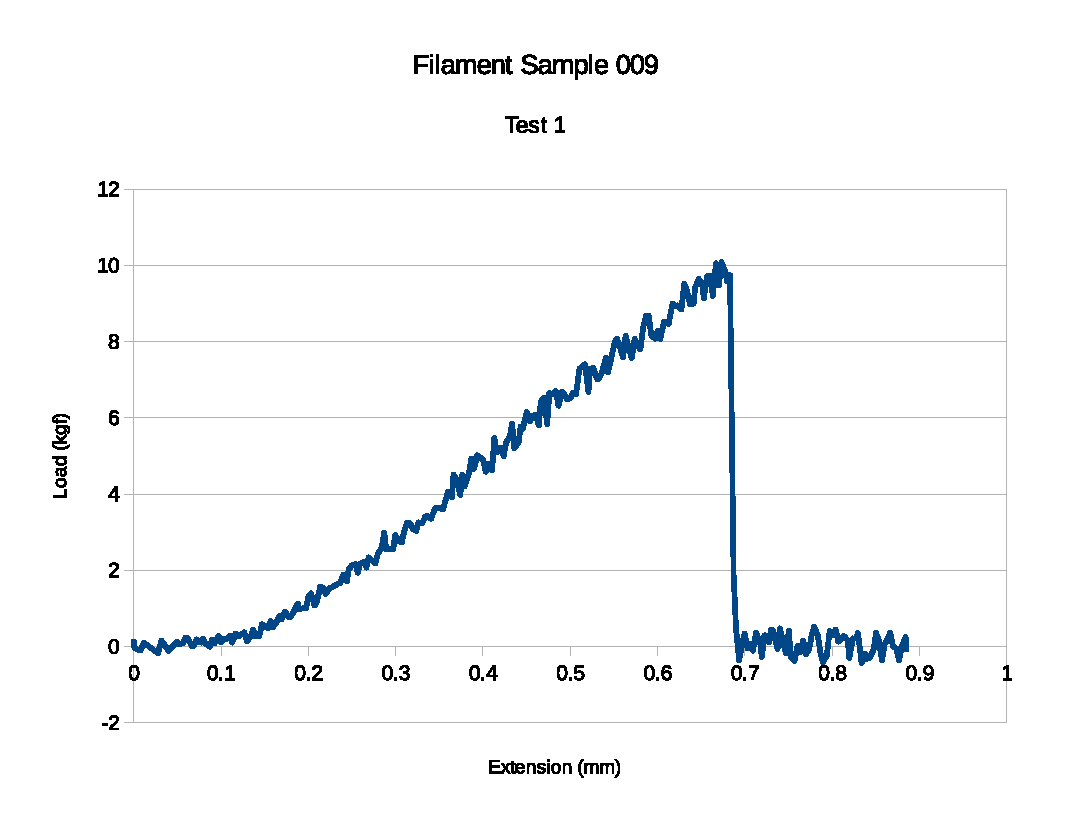
\includegraphics[width=0.8\textwidth]{./figures/009T1-instron-data}
    \caption{Sample tensile test data for a slurry-dipped filament sample.}
    \label{fig:instron-sample}
\end{figure}

\begin{table}[h]
    \centering
    \begin{tabular}{lcccc}
        Material           & Ultimate Tensile Strength (MPa)   & Stiffness (GPa)    & Density ($ kg/m^{3} $)  \\ \hline
        ABS                & 53                                & 2.3                & 1040 \\
        Carbon Fiber       & 3750                              & 231                & 1750 \\
        Aluminum 6061      & 310                               & 68.9               & 2700 \\
        Pultruded Filament & 313                               & 13.4               & 1354 \\ 
        Dipped Filament    & 690                               & 19.6               & 1567 \\
    \end{tabular}
    \caption{Preliminary CFRP filament test results, as compared to its constituents and to aluminum.}
    \label{tab:test-results}
\end{table}

\clearpage

\subsection{Print Testing}

\indent

\begin{figure}[h!]
        \centering
        \begin{subfigure}[b]{0.45\textwidth}
                \includegraphics[width=\textwidth]{./figures/filament-print-3doodler-before}
                \caption{Before.}
                \label{fig:filament-print-3doodler-before}
        \end{subfigure}
        \begin{subfigure}[b]{0.45\textwidth}
                \includegraphics[width=\textwidth]{./figures/filament-print-3doodler-after}
                \caption{After.}
                \label{fig:filament-print-3doodler-after}
        \end{subfigure}
        \caption{Before and after shots of print testing with the CFRP filament.}\label{fig:filament-print-test}
\end{figure}

\begin{figure}[htp]
    \centering
    \includegraphics[width=0.5\textwidth]{./figures/filament-print-3doodler-during}
    \caption{Test printing the CFRP filament with a 3Doodler.}
    \label{fig:filament-print-3doodler-during}
\end{figure}

\begin{figure}[htp]
    \centering
    \includegraphics[width=0.8\textwidth]{./figures/filament-extrude}
    \caption{A close up photo of the filament printed with the 3Doodler}
    \label{fig:filament-extrude}
\end{figure}